%!TEX root =  main.tex
\appendix
\chapter{Detailed List of Self-Healing Approaches}
\label{ap:approches}

This appendix reports \ldots 

\section{} \label{}
\begin{compactitem}
\item[\textbf{Title}]Self-Adapting Reliability in Distributed Software Systems
\item[\textbf{Author}] 
Brun et al.
\item[\textbf{Reference}] 
\cite{brun_self-adapting_2015}
\item[\textbf{Year}] 
August, 2015
\item[\textbf{Application Domain}] 
Distributed computation architecture
\item[\textbf{Self-Healing steps}] Self-healing steps involved are fault-detecting, diagnosis and recovering
\item[\textbf{Technical Approach}]Iterative redundancy technique
\item[\textbf{Basic Idea}] 

The iterative redundancy algorithm is used to calculate the minimum of jobs to get a consensus, assuming that all the jobs produce the same result. The minimum number of jobs $d$ is calculated taking into account the system reliability $\mathbb{R}$ and node reliability $r$. The system reliability is used as a confidence threshold.

The minimum number of jobs $d$ is calculated taking into account the system reliability $\mathbb{R}$ and node reliability $r$, using the formulae:


\begin{figure}[H]
\center
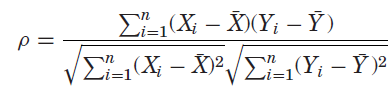
\includegraphics[width=1.5in]{img/formulae}
\caption{The reliability of a system:}
\end{figure} 





\item[\textbf{Summary of approach}]


Distributed computing architectures ensure the correct execution of each task through voting: multiple independent computational nodes perform the same task and if the majority of executions agree on a result, a consensus exists, and that result is taken to be the solution of that task. Iterative redundancy tries to optimize the use of computational nodes by distributing the minimum number of jobs that perform the same task required to achieve a desired confidence level in the result, assuming that all the jobs’ results agree. Then, if all jobs agree, the task is completed. However, if some results disagree, the confidence level associated with the majority result is diminished because of the chance that the disagreeing results are correct. The proposed approach then reevaluates the situation and distributes the minimum number of additional jobs that would achieve the desired level of confidence.
This process repeats until the agreeing results sufficiently outnumber the disagreeing results to reach the confidence threshold.


The flow-digram of the iterative redundancy algorithm is given by:
\begin{figure}[H]
\center
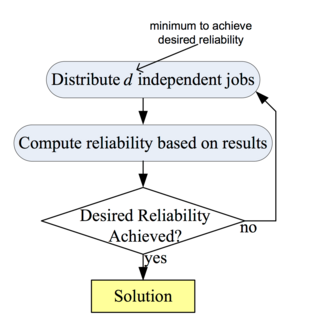
\includegraphics[width=5in]{img/Iterativeredundancyschematic}
\caption{Iterative redundancy schematic:}
\end{figure} 

\item[\textbf{Fault Types}]Byzantine attacks: A Byzantine fault is one where the faulty unit continues to run but produces incorrect results and might lead to failure sometimes.

\item[\textbf{Failure Types}]Byzantine attacks.

\item[\textbf{Input data}] n independent jobs that perform the same jobs.

\item[\textbf{Recovery actions}]The technique try the deploy the redundant number of jobs in order to achieve consensus level.

\item[\textbf{Advantages}] Iterative redundancy is more cost effective as it creates the same level of software system reliability at a lower expense.

\item[\textbf{Disadvantages}] In iterative redundancy, the task server deploys several jobs and wait for the responses before possibly choosing to deploy more jobs. Therefore, this technique increases the latency for a particular task.

\item[\textbf{Case studies}]
The technique is implemented and tested on PlanetLab. PlanetLab is a gathering of PCs accessible as a testbed for distributed systems research.\\
\end{compactitem}


\begin{compactitem}
\item[\textbf{Title}]SH˜oWA: A Self-Healing Framework for Web-Based

\item[\textbf{Author}]Magalhães and Silva 

\item[\textbf{Reference}]

\cite{magalhaes_showa:_2015}

\item[\textbf{Year}] 2015

\item[\textbf{Application Domain}]
Web-based applications 

\item[\textbf{Self-Healing steps}] 
The self-healing loop used in this paper has four stages:Monitor, Plan, Analyze and Execute.

\item[\textbf{Technical Approach}]Aspect oriented programming, Pearson's and Spearman's rank correlation analysis.

\item[\textbf{Basic Idea}] 
Detects anomalies in web applications by statistical correlation analysis. Uses data analysis techniques to detect variations in server response time and finds out whether the change of time was due to work load or degradation in performance. If the delay in response time was due to performance anomaly, then respective recovery strategies is executed autonomously.

\item[\textbf{Summary of approaches}] 

1.Aspect oriented programming is used build up the sensor module to collect data and response time at runtime.\\

2.The parameters collected is analysed using Pearson's correlation coefficient (X = the sequence of the accumulated response server time per user transaction and Y= the number of user transactions processed in the same interval) to calculate the degree of association (p), which determines  the chances of anomaly.More correlation = chances of more anomaly and less correlation = chances of less anomaly.\\

3.We use Spearman's rank correlation to measure the degree of association between X and Y, denoted by rho(ρ). If ρ is stable / high across,then the response time is associated with the application workload and if ρ decreases, the response time delay is due to performance anomaly.\\

4. In the workload variation analysis module, the input for this module are: X=Accumulated response time in a given time interval and Y= The total number of requests waiting in the application container queue in the same time interval.We calculate ρ using spearman’s rank correlation coefficient.The fact that the ρ degree is low and stable means two things: (1) the response time has not suffered delays, and (2) there was no significant accumulation of requests in the application server queue waiting to be processed. If the ρ degree is medium or large, then it means that there are problems with the processing workload. The several workload problems are (e.g., bursty workload, server queue issues).\\

5. In the anomaly detector module, after detecting a performance anomaly, the anomaly detector modules aims to identify, if there is any system or application server change associated with the anomaly. X= The total number of user transactions processed in an interval and Y=The accumulated value of the parameters collected by the sensor module in the same interval. Y is a vector which contains each parameter collected. ρ degree will decrease or constant, showing the parameters (or set of parameters) is no longer associated with the number of requests.In this case, no changes in the correlation degree between the parameters that are analyzed and the number of user transactions processed.It can be said that the performance anomaly is not related to changes at the system or application server level.\\

6. The root-cause failure analysis module analyzes the user transactions that have reported only a performance anomaly. To verify if a performance anomaly is associated with an application change or a remote service change, X is defined as the frequency distribution of the transaction response time and Y assumes the response time frequency distribution of the calls belonging to the transaction call path. The correlation between the variables is determined using Spearman’s rank correlation coefficient. In this situation, the ρ degree increases, highlighting the calls potentially associated with the performance slowdown.\\

7. The recovery planner module is used to store the recovery procedure. The executor module is responsible for executing the specific recovery actions that has been triggered. The method is implemented using a client-server program. The client sends the actions to be performed to the server and receives feedback about its implementation. The semisupervised methodology makes use of utility functions and machine learning techniques to select a recovery procedure for a  particular anomaly. In the current implementation, the recovery process is procedure based and defined by a human operator.

\item[\textbf{Fault types}]Response time delay from the application server

\item[\textbf{Failures types}]Response time delay from the application server

\item[\textbf{Input data}] The input are the parameters which are collected by the sensor module. For instance user transactions, CPU time per user transactions, amount of available memory.

\item[\textbf{Recovery actions}]The output are the recovery strategies which are carried forward or executed against the particular anomalies detected.

\item[\textbf{Advantages}] It is advantageous of the showa sensor module is that it separates the monitoring code from the application code, thereby allowing an application to be monitored without the need for manually changing its source code. With this separation, multiple applications can be monitored using the same monitoring code.

The framework is generic and can be applied to any type of transactional Web application. The only module that needs to be ported is the Sensor module

\item[\textbf{Disadvantages}]The ability to detect anomalies while the number of end users affected is low.

\item[\textbf{Case studies}]One retail store web application and an auction web application has been used in this paper for testing the framework.
\end{compactitem}



\begin{compactitem}
\item[\textbf{Title}]GenProg: A Generic Method for Automatic Software Repair

\item[\textbf{Author}]
Goues et al.   
\item[\textbf{Reference}]  

\cite{le_goues_genprog:_2012}

\item[\textbf{Application Domain}]
Real, unannotated programs with publicly documented bugs

\item[\textbf{Self-Healing steps:}]. The closed loop repair system works in this way. The method adopts an IDS (intrusion-detection system) that detects the anomalies in the system.

Whenever, the Intrusion Detection System,IDS detects an annomaly, GenProg is invoked to repair the suspicious behavior.

\item [\textbf{Technical Approach}] The method adopts an IDS (intrusion-detection system) that detects the anomalies in the system.

\item[\textbf{Basic Idea}] The program implements three functions:

The \textit{initialpopulation} generates the variants by using the mutual operators based on the input program and test cases.

The \textit{fitness function} evaluates each variants created and chooses the best amongst them.

The \textit{GenProg} iterates by selecting high fitness individuals, which are selected for continuous evolutions for the next.

\item[\textbf{Summary of approach}]
The technical approach used in this paper by the author can be classified in four stages:-
\textit{Program Representation:}Each variant is represented by a pair of an abstract syntax tree   (AST)and a weighted path. The abstract syntax tree contains all the statements of the program and a weighted path contains all the statements in the program that has been assigned a weight based on the occurrence of the statement the test cases.\\

\textit{Selection and Genetic Operators:}GenProg discards individuals with fitness 0 (variants that do not compile or that pass no test cases) and places the remainder in Viable. It then uses a selection strategy to select pop size/2 members of a new generation from the previous iteration.\\ 

\textit{Fitness function:}The fitness function evaluates the acceptability of a program variant. The fitness function mentioned in this paper, encodes software requirements at the test case level: negative test cases encode the fault to be repaired, while positive test cases encode functionality that cannot be sacrificed.\\

\textit{Repair Minimization:}

The search terminates successfully when GP discovers a primary repair that passes all test cases. Due to randomness in the mutation and crossover algorithms, the primary repair typically contains at least an order-of-magnitude more changes than are necessary to repair the program, rendering the repairs difficult to inspect for correctness.


\item[\textbf{Fault Types}]Infinite loop, Segmentation fault, Remote heap buffer over flow to inject code, Remote heap buffer overflow to overwrite variables, Non overflow denial of service, Local stack buffer overflow, Integer overflow and Format string vulnerability.

\item[\textbf{Input data}] Input source code contains a failing negative test case that exercises the defect and a set of passing positive test cases that describe requirements.

\item[\textbf{Recovery actions}]The recovery action is the primary repair that passes all test cases.

\item[\textbf{Advantages}] 
The GP search space focuses genetic operations along a weighted path and takes advantage of test case coverage information, and reusing existing program statements.

\item[\textbf{Disadvantages}] GenProg relies on test cases to encode both an error to repair and important functionality. GenProg cannot repair race conditions as it is difficult to encode an error using test cases for non-deterministic properties.


\end{compactitem}



\begin{compactitem}

\item[\textbf{Title}]Exception Handling for Repair in Service-Based Processes

\item[\textbf{Author}]Friedrich et al.

\item[\textbf{Reference}] 

\cite{friedrich2010exception}

\item[\textbf{Year}] 2010

\item[\textbf{Application Domain}]
Service-based processes

\item[\textbf{Self-Healing steps}] The self healing loop is: design, diagnosis, repair


Diagnosis: This phase determines where the error took place and what the cause of the error is. The knowledge about the fault is crucial for repairing the process and for minimizing the need for re executing parts of the process. Such knowledge is obtained through diagnosis,  using a diagnosis tool.

\item[\textbf{Technical Approach}]Model based approach

\item[\textbf{Basic Idea}] In this paper, we design repair strategies based on the structure of the process by using model-based approach. The repair plan / actions is defined in the process model. The approach is based on the concept of self-healing system. In this approach, the repair information is associated with a process at design time and the repair plans are generated at runtime.

\item[\textbf{Summary of approach}]

\item[\textbf{Fault Types}]The two types of faults that can be healed in this case are: 

\item[\textbf{Failure Types}]The two types of faults that has been healed in this case are:

An incorrect item code with an item name. The system send a wrong shipping note to warehouse, which therefore does not process the order and the package correctly.


When the are house receives the item description from the SHOP through the FORWARDORDER operation, it discovers that the order goods, the shipping note and the package are inconsistent with respect to the goals provided by the supplier and thus raised failure 1.

\item[\textbf{Input data}] 

\item[\textbf{Recovery actions}]

\item[\textbf{Advantages}] 
Repair follows the same logic as the original process and different repairs can be proposed for different causes of failures, with the goal of minimizing both the amount of work to be redone in the process and the compensation and/or reexecution of external services.

\item[\textbf{Disadvantages}] 



\item[\textbf{Case study}] 


The approach has been used on a food shop selling company, which sells products online using a service-oriented architecture (SDA) infrastructure with four services.

\end{compactitem}




